\documentclass[compress,red]{beamer}
\usepackage[utf8]{inputenc}
\usepackage{ucs}
\usepackage{amsmath}
\usepackage{amsfonts}
\usepackage{amssymb}
\usepackage[russian]{babel}
\usepackage{graphicx}
\usepackage{wrapfig}

\usepackage{tikz}
\usepackage{verbatim}

\usepackage{color}
\usepackage{xcolor}
\usepackage{listings}

\usepackage{caption}

\lstset{
language=ruby,
extendedchars=\true,
inputencoding=utf8x,
commentstyle=\itshape,
stringstyle=\bf,
belowcaptionskip=5pt }


\DeclareCaptionFont{white}{\color{white}}
\DeclareCaptionFormat{listing}{\colorbox{gray}{\parbox{\textwidth}{#1#2#3}}}
\captionsetup[lstlisting]{format=listing,labelfont=white,textfont=white}

\usetikzlibrary{calc,trees,positioning,arrows,chains,shapes.geometric,%
    decorations.pathreplacing,decorations.pathmorphing,shapes,%
    matrix,shapes.symbols}

\tikzset{
>=stealth',
  punktchain/.style={
    rectangle, 
    rounded corners, 
    % fill=black!10,
    draw=black, very thick,
    text width=10em, 
    minimum height=3em, 
    text centered, 
    on chain},
  line/.style={draw, thick, <-},
  element/.style={
    tape,
    top color=white,
    bottom color=blue!50!black!60!,
    minimum width=8em,
    draw=blue!40!black!90, very thick,
    text width=10em, 
    minimum height=1.5em, 
    text centered, 
    on chain},
  every join/.style={->, thick,shorten <=1pt},
  decoration={brace},
  tuborg/.style={decorate},
  tubnode/.style={midway, right=2pt},
}

\mode<presentation>

\usetheme{Warsaw}

\definecolor{Red}{rgb}{1,0,0}
\definecolor{Blue}{rgb}{0,0,1}
\definecolor{Green}{rgb}{0,1,0}
\definecolor{magenta}{rgb}{1,0,.6}
\definecolor{lightblue}{rgb}{0,.5,1}
\definecolor{lightpurple}{rgb}{.6,.4,1}
\definecolor{gold}{rgb}{.6,.5,0}
\definecolor{orange}{rgb}{1,0.4,0}
\definecolor{hotpink}{rgb}{1,0,0.5}
\definecolor{newcolor2}{rgb}{.5,.3,.5}
\definecolor{newcolor}{rgb}{0,.3,1}
\definecolor{newcolor3}{rgb}{1,0,.35}
\definecolor{darkgreen1}{rgb}{0, .35, 0}
\definecolor{darkgreen}{rgb}{0, .6, 0}
\definecolor{darkred}{rgb}{.75,0,0}

\xdefinecolor{olive}{cmyk}{0.64,0,0.95,0.4}
\xdefinecolor{purpleish}{cmyk}{0.75,0.75,0,0}

\useoutertheme[subsection=false]{smoothbars}

\title{Построение диаграмм и задачи}

%\usecolortheme{dolphin}


\begin{document}
%%титульная страница
\maketitle
%% основные моменты

\section{Диаграммы}

\subsection{Диаграммы}
\begin{frame}[fragile]
  \frametitle{Диаграммы}
  \begin{itemize}
      \item Диаграммы --- способ визуализации данных.
      \item Они показывают зависимость одной величины от другой, соотношение величин и др.
      \item Есть разные типы диаграмм: начиная от простых графиков и заканчивая сложными географическими картами.
      \item Google Drive поддерживает огромное множество решений.
  \end{itemize}
\end{frame}

\subsection{Диаграмма 1}
\begin{frame}[fragile]
  \frametitle{Создание диаграммы}
  \centerline{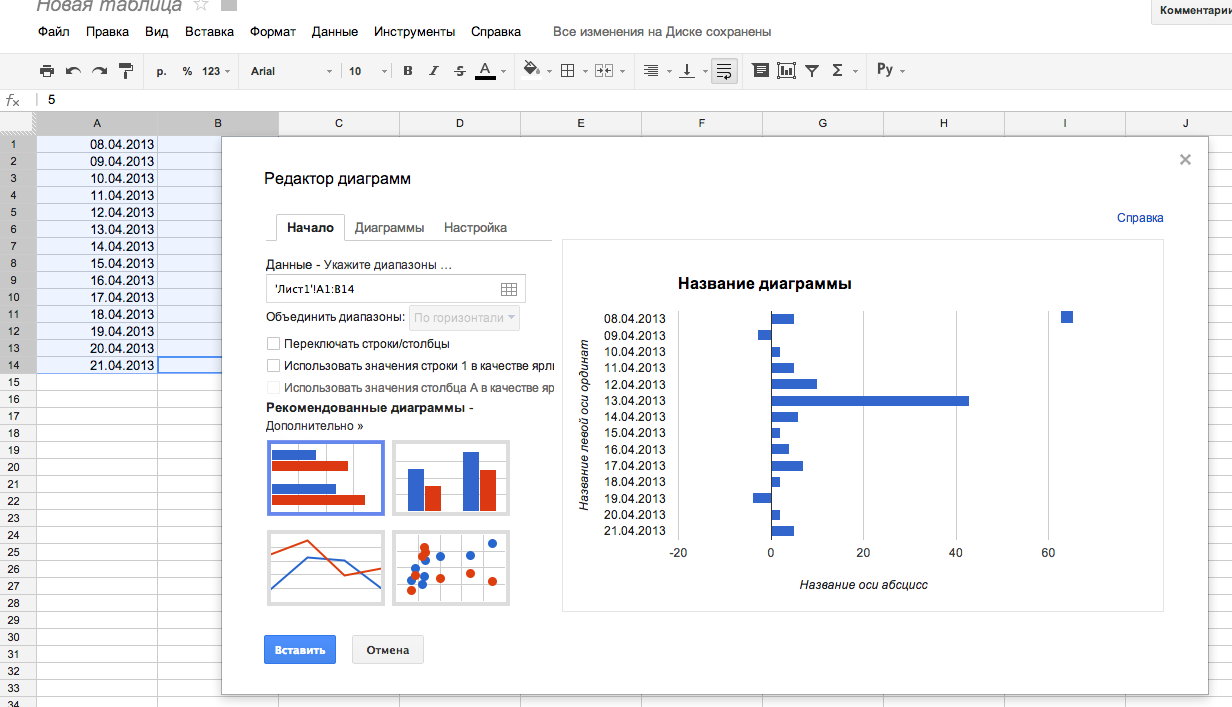
\includegraphics[width=0.8\textwidth]{images/02.png}}
  \begin{itemize}
      \item Для создания диаграммы выделите нужный участок данных и нажмите на кнопку ``Вставить диаграмму''
  \end{itemize}
\end{frame}

\subsection{Выбор типа}
\begin{frame}[fragile]
  \frametitle{Выбор типа диаграммы}
  \centerline{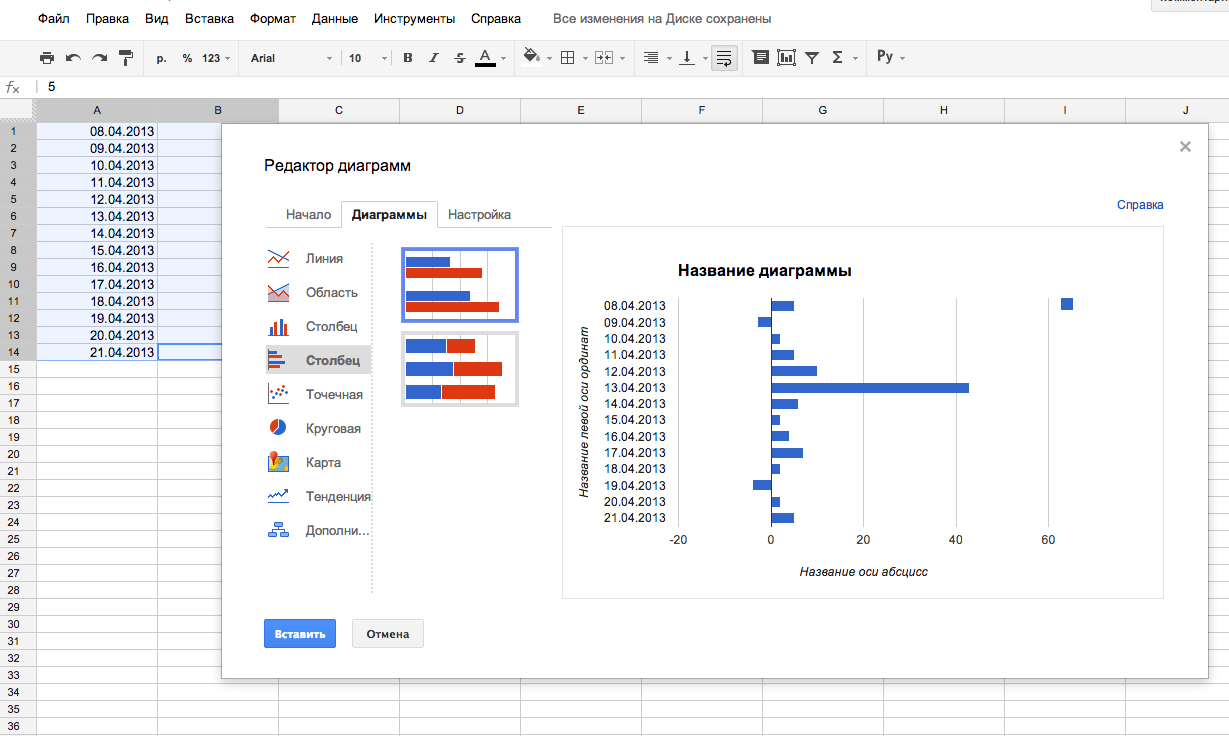
\includegraphics[width=0.8\textwidth]{images/03.png}}
  \begin{itemize}
      \item Вторая вкладка --- выбор типа диаграммы.
      \item \textbf{NB}: диаграмма--``столбцы'' называется \emph{гистограмма}.
  \end{itemize}
\end{frame}

\subsection{Выбор типа 2}
\begin{frame}[fragile]
  \frametitle{Выбор типа диаграммы}
  \centerline{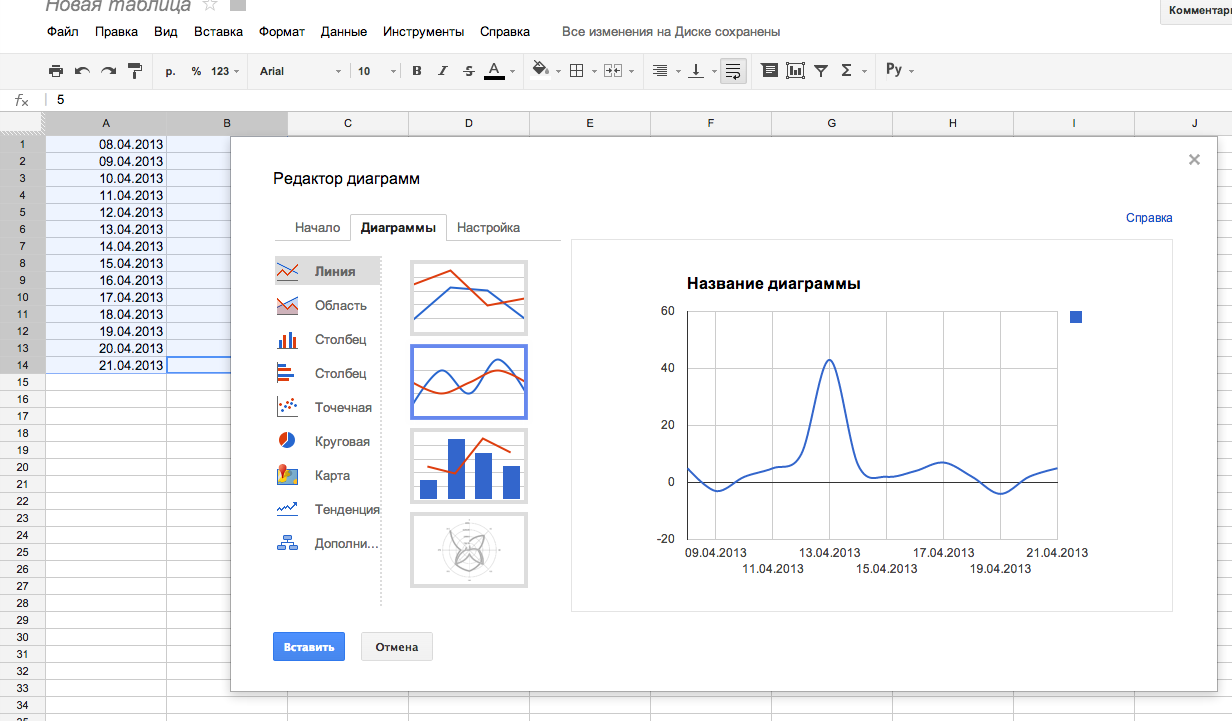
\includegraphics[width=0.8\textwidth]{images/03-2.png}}
  \begin{itemize}
      \item Выберем сглаженный график.
  \end{itemize}
\end{frame}

\subsection{Настройка}
\begin{frame}[fragile]
  \frametitle{Настройка диаграммы}
  \centerline{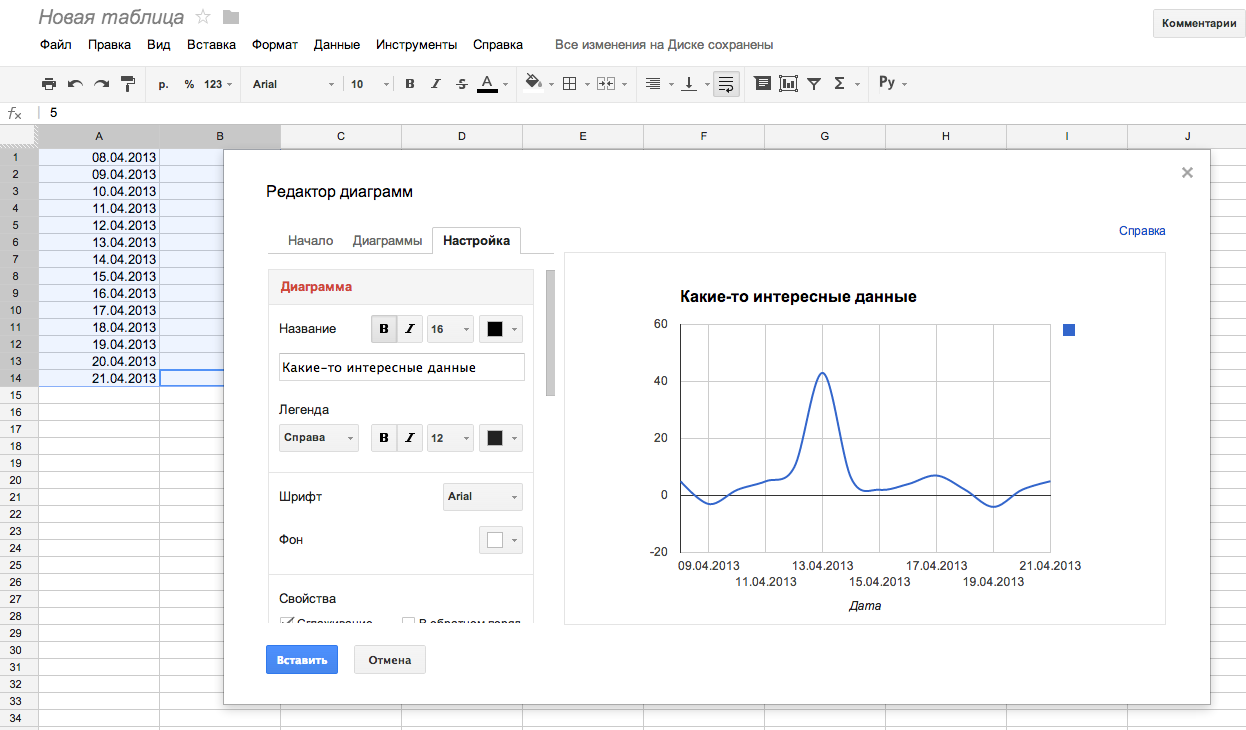
\includegraphics[width=0.8\textwidth]{images/04.png}}
  \begin{itemize}
      \item В третьей вкладке можно указать название диаграммы, названия осей, цвета, расположение и пр.
  \end{itemize}
\end{frame}

\subsection{Перемеещение}
\begin{frame}[fragile]
  \frametitle{Перемещение диаграммы}
  \centerline{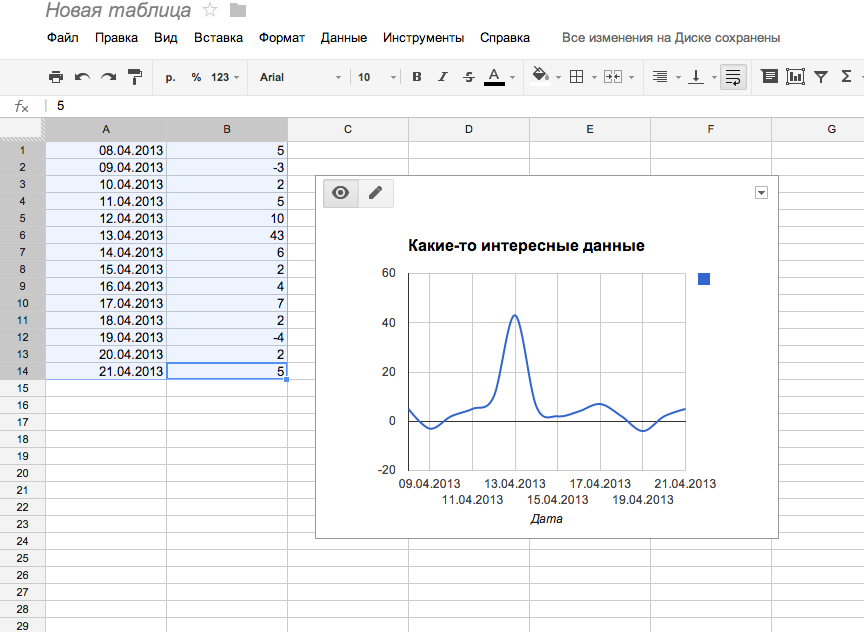
\includegraphics[width=0.6\textwidth]{images/05.png}}
  \begin{itemize}
      \item Диаграмму можно редактировать в режиме ``редактирования'' (карандашик) и перетаскивать в режиме ``просмотр'' (глаз).
  \end{itemize}
\end{frame}

\subsection{Пример круговой диаграммы}
\begin{frame}[fragile]
  \frametitle{Пример круговой диаграммы}
  \centerline{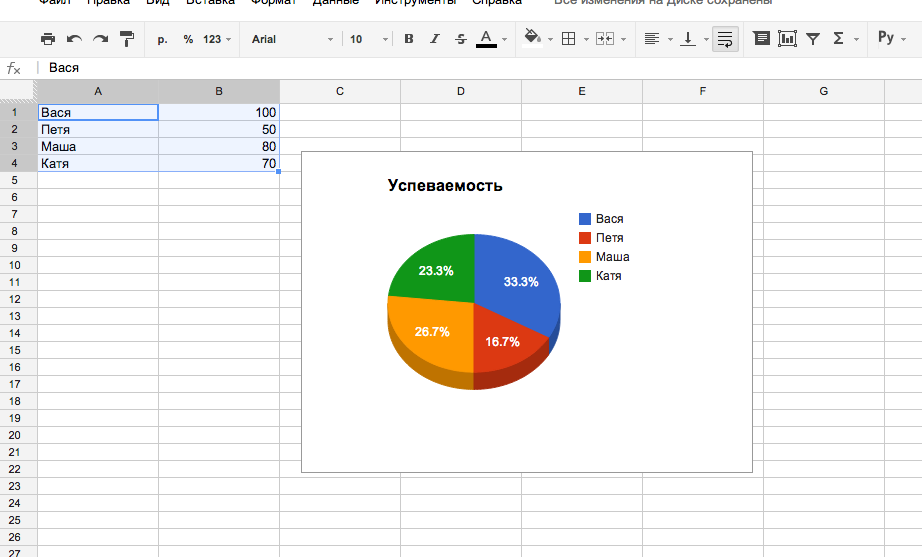
\includegraphics[width=0.8\textwidth]{images/06.png}}
\end{frame}

\section{Задачи}
\subsection{Задачи на диаграммы}
\begin{frame}
  \begin{center}
    \Huge{Задачи}
  \end{center}
  \begin{center}
    \Large{на диаграммы}
  \end{center}
\end{frame}

\subsection{Задача 1}
\begin{frame}[fragile]
  \frametitle{Задача 1}
  \centerline{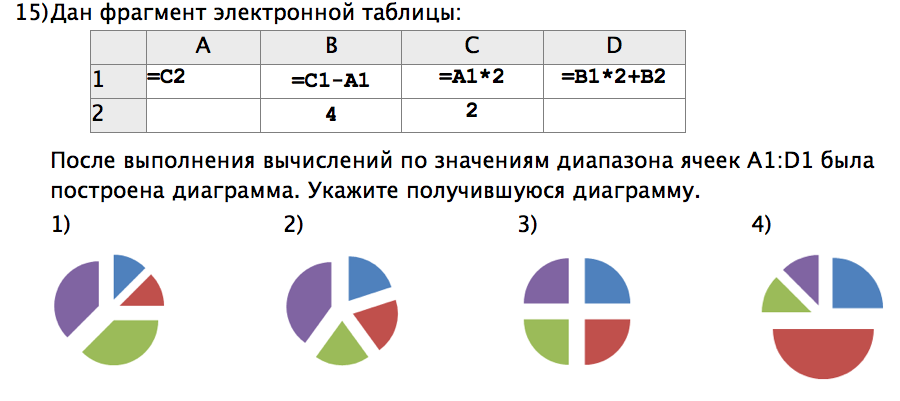
\includegraphics[width=1.0\textwidth]{images/07.png}}
\end{frame}

\subsection{Задача 1-2}
\begin{frame}[fragile]
  \frametitle{Задача 1}
  \centerline{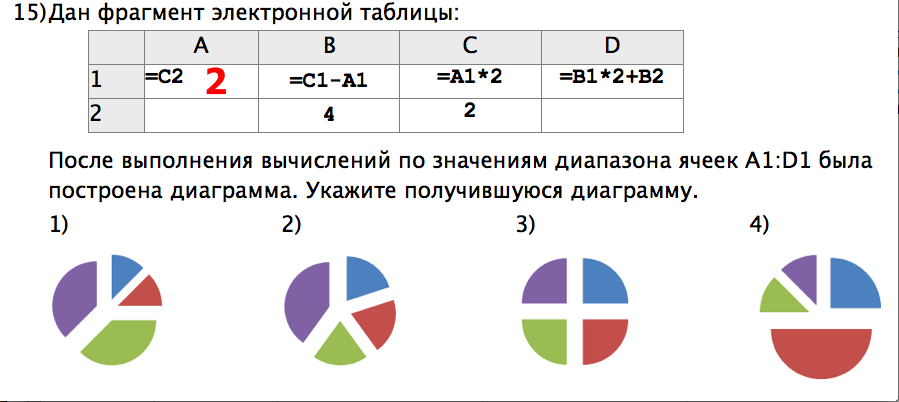
\includegraphics[width=0.8\textwidth]{images/07-1.png}}
  \begin{itemize}
      \item Вычислим те значения, которые нам известны. A1 --- очевидно.
  \end{itemize}
\end{frame}

\subsection{Задача 1-3}
\begin{frame}[fragile]
  \frametitle{Задача 1}
  \centerline{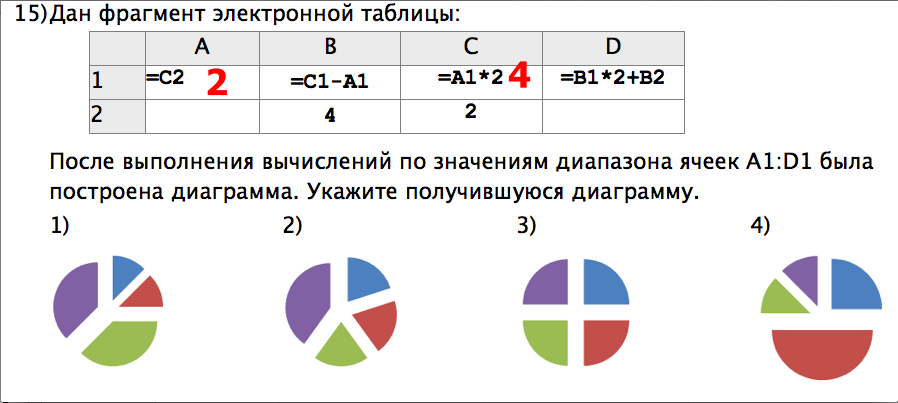
\includegraphics[width=0.8\textwidth]{images/07-2.png}}
  \begin{itemize}
      \item Теперь C1.
  \end{itemize}
\end{frame}

\subsection{Задача 1-4}
\begin{frame}[fragile]
  \frametitle{Задача 1}
  \centerline{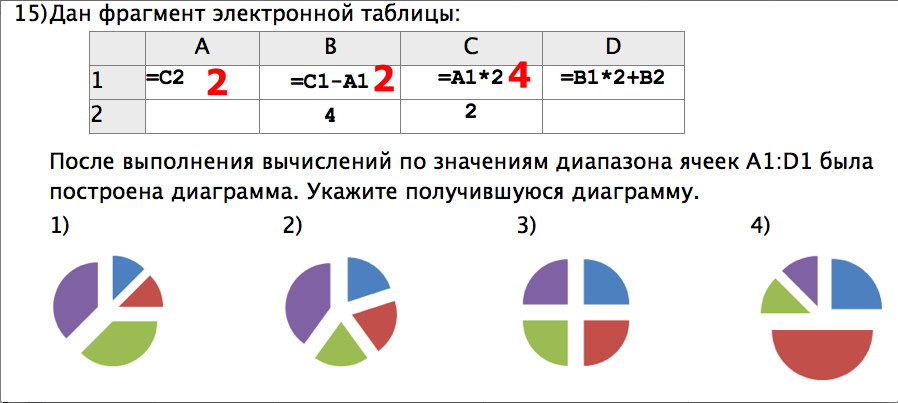
\includegraphics[width=0.8\textwidth]{images/07-3.png}}
  \begin{itemize}
      \item Теперь B1.
  \end{itemize}
\end{frame}

\subsection{Задача 1-53}
\begin{frame}[fragile]
  \frametitle{Задача 1}
  \centerline{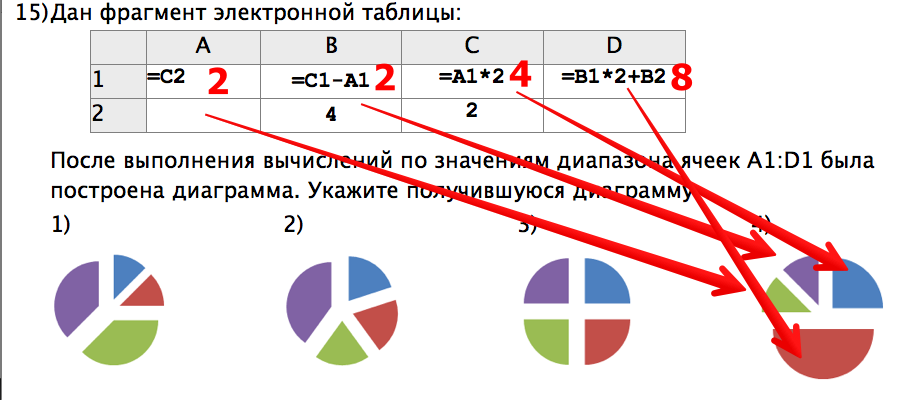
\includegraphics[width=0.8\textwidth]{images/07-4.png}}
  \begin{itemize}
      \item Теперь D1. Итого, имеем: 2 одинаковых, одна --- в два раза больше и ещё одна в 2 раза больше предыдущей.
      \item Подходит ответ №4.
  \end{itemize}
\end{frame}

\subsection{Задача 2}
\begin{frame}[fragile]
  \frametitle{Задача 2}
  \centerline{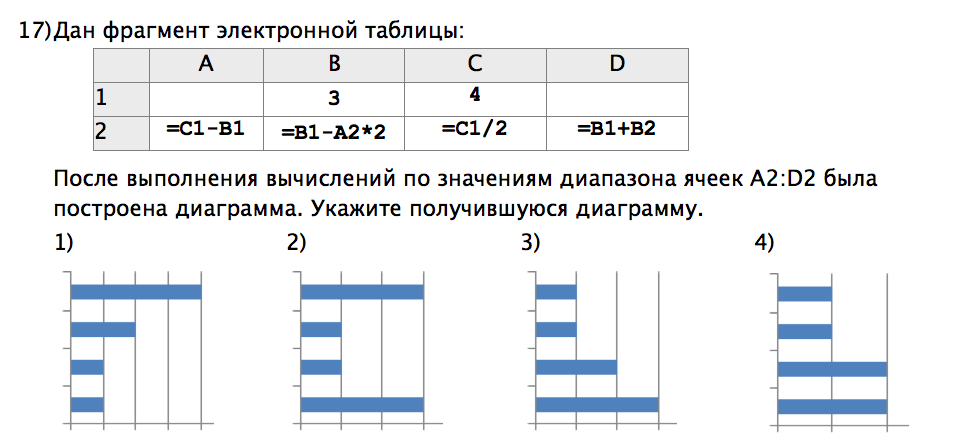
\includegraphics[width=1.0\textwidth]{images/08.png}}
\end{frame}

\subsection{Задача 2-1}
\begin{frame}[fragile]
  \frametitle{Задача 2}
  \centerline{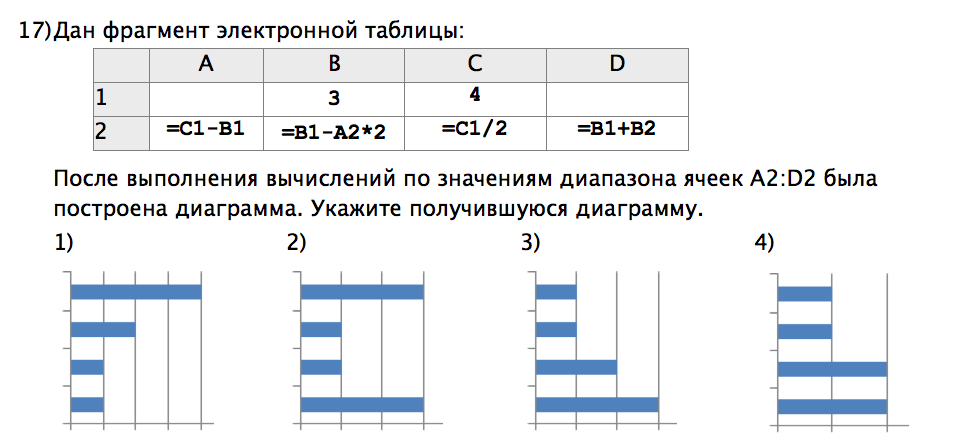
\includegraphics[width=1.0\textwidth]{images/08.png}}
  \begin{itemize}
      \item Ответ: 1.
  \end{itemize}
\end{frame}

\subsection{Задача 3}
\begin{frame}[fragile]
  \frametitle{Задача 3}
  \centerline{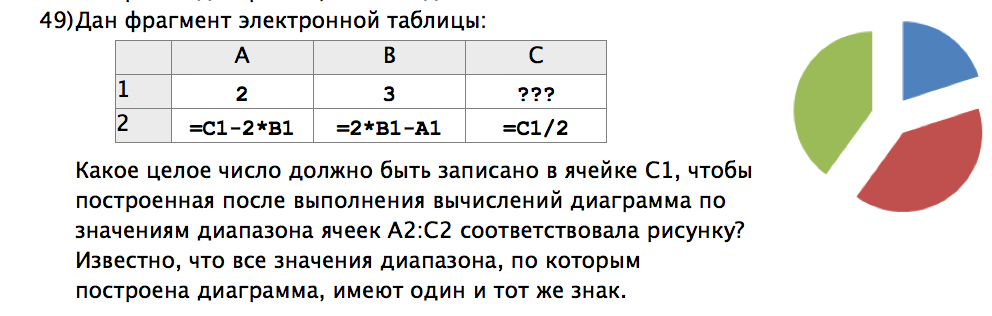
\includegraphics[width=1.0\textwidth]{images/09.png}}
\end{frame}

\subsection{Задача 3-2}
\begin{frame}[fragile]
  \frametitle{Задача 3}
  \begin{itemize}[<+->]
    \item Рассмотрим внимательно диаграмму. На ней есть: маленькая ячейка и две равные, в два раза превышающие маленькую. 
    \item Значит, от A2 до C2 --- два равных числа и ещё одно, в два раза меньшее.
    \item B2: =2*B1-A1 =6-2 = 4
    \item A2: =C1-2*B1 = C1-6
    \item Возможны три ситуации: A2=B2, A2=C2, B2=C2.
    \item $A2=B2: C1-6=4$. Значит, C1=10. Значит, в C2: 10/2=5. Не подходит.
    \item $A2=C2: C1/2=C1-6 => C1=2C1-12 => C1=12$. Не сходится.
    \item Значит, $B2=C2: C1/2=4 => C1=8$. 
  \end{itemize}
\end{frame}

\subsection{Задача 4}
\begin{frame}[fragile]
  \frametitle{Задача 4}
  \centerline{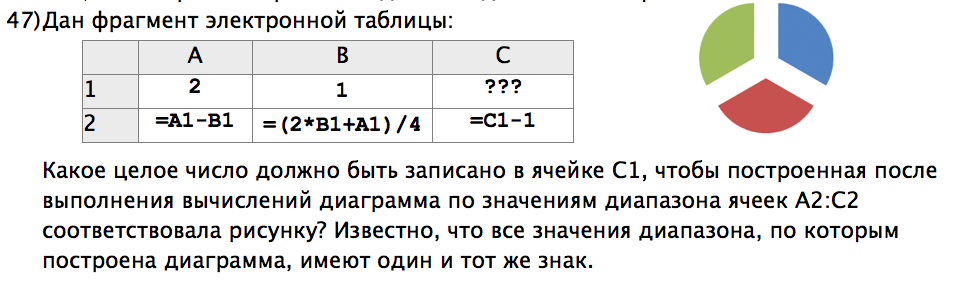
\includegraphics[width=1.0\textwidth]{images/10.png}}
\end{frame}

\subsection{Задача 4-1}
\begin{frame}[fragile]
  \frametitle{Задача 4}
  \centerline{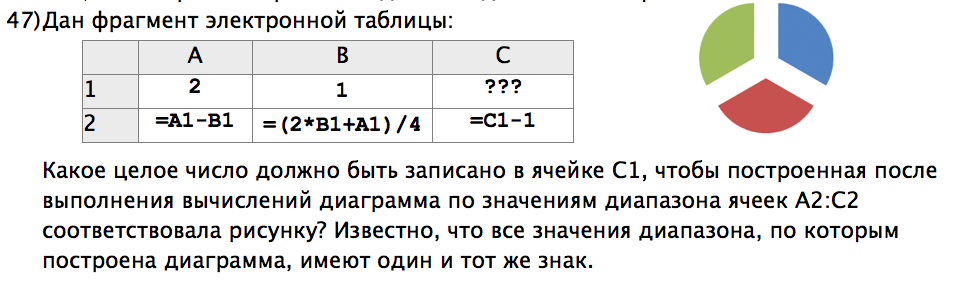
\includegraphics[width=1.0\textwidth]{images/10.png}}
  \begin{itemize}
      \item Ответ: 2.
  \end{itemize}
\end{frame}

\subsection{Задача 5}
\begin{frame}[fragile]
  \frametitle{Задача 5}
  \centerline{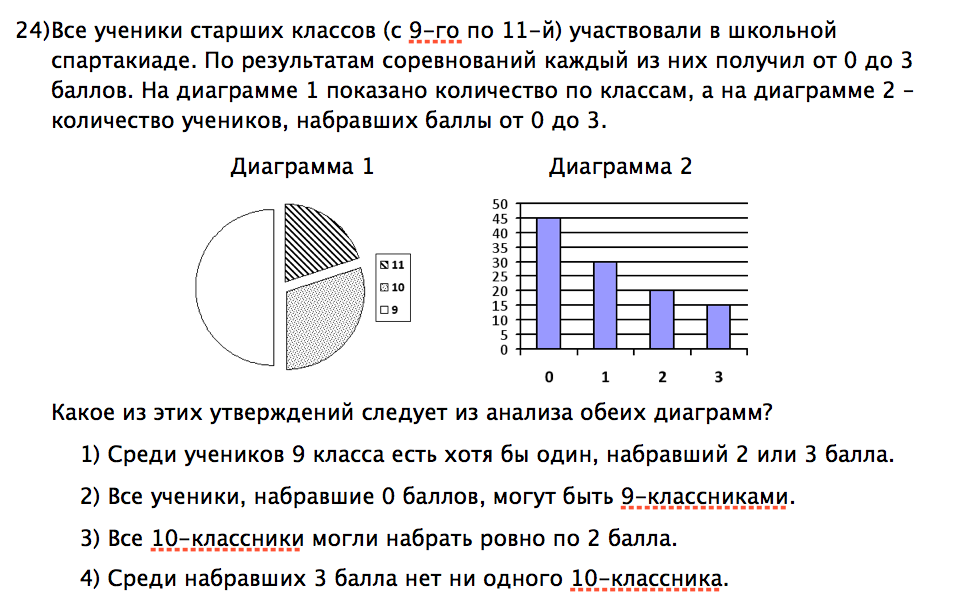
\includegraphics[width=0.9\textwidth]{images/11.png}}
  \begin{itemize}
      \item Решение через рассуждение.
  \end{itemize}
\end{frame}

\subsection{Задача 6}
\begin{frame}[fragile]
  \frametitle{Задача 6}
  \centerline{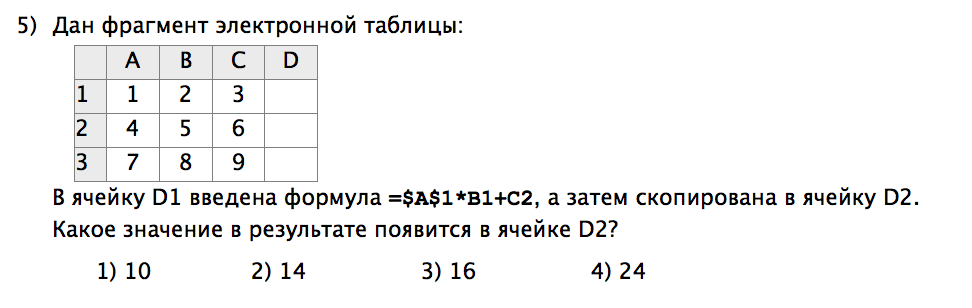
\includegraphics[width=0.9\textwidth]{images/12.png}}
  \begin{itemize}
      \item Абсолютная и относительная адресации.
  \end{itemize}
\end{frame}

\subsection{Задача 7}
\begin{frame}[fragile]
  \frametitle{Задачи 7-9}
  \begin{itemize}[<+->]
    \item \textbf{Задача 7.} В электронной таблице значение формулы =СРЗНАЧ(A6:C6) равно (-2). Чему равно значение формулы =СУММ(A6:D6), если значение ячейки D6 равно 5? 
    \item \textbf{Задача 8.} В электронной таблице значение формулы =СУММ(C3:E3) равно 15. Чему равно значение формулы =СРЗНАЧ(C3:F3), если значение ячейки F3 равно 5?
    \item \textbf{Задача 9.} В электронной таблице значение формулы =СРЗНАЧ(A1:C1) равно 5. Чему равно значение ячейки D1, если значение формулы =СУММ(A1:D1)равно 7?
  \end{itemize}
\end{frame}

\subsection{Разбор задачи 7}
\begin{frame}[fragile]
  \frametitle{Разбор задачи 7}
  \begin{itemize}[<+->]
    \item Разберём задачу 7.
    \item Что такое =СРЗНАЧ(A6:C6) = -2?
    \item $\cfrac{\mathrm{A6+B6+C6}}{3} = -2$.
    \item Следовательно, $\mathrm{A6+B6+C6} = -6$.
    \item Что такое =СУММ(A6:D6)?
    \item $\mathrm{A6+B6+C6+D6 = (A6+B6+C6) + 5 = -6 + 5 = -1}$.
  \end{itemize}
\end{frame}

\subsection{Благодарности}
\begin{frame}[fragile]
  \frametitle{Благодарности}
  \begin{itemize}
    \item Спасибо сайту http://kpolyakov.spb.ru/ за предоставленные задачи для ЕГЭ.
  \end{itemize}
\end{frame}

\end{document}